\chapter{SMartyTesting}
\label{sec:abordagem}
\pagestyle{plain}

\section{Considerações Iniciais}

Neste capitulo é apresentado uma abordagem que auxilia na geração de sequências de teste em tempo de modelagem, dentro da engenharia de domínio a partir de modelos UML. Tais sequências de teste poderão ser utilizadas para a geração de casos de teste, que em um segundo momento poderão ser aplicados na engenharia de aplicação. Denominada \textit{SMartyTesting}, um perfil de validação \textit{SMarty}, tem por objetivo auxiliar o arquiteto de software com a geração de sequências de teste a partir de diagramas de sequência, onde o diagrama é convertido para máquina de estado, após este processo é realizado a geração da sequência de teste, isso é feito para todos os produtos derivados de uma linha de produto de software, considerando suas variabilidades.

Para esta seção ser mais produtiva recomendamos a leitura da Seção \ref{sec:fundamentacao}, logo em seguida conhecer mais sobre a abordagem de gerenciamento de variabilidade \textit{SMarty},   

\section{Caracterização da Abordagem SMartyTesting}
\label{caracterizacao_smarty}

\subsection{Motivação de Pesquisa}

Apesar de teste de software ser altamente difundido, assim como o conceito de LPS, sempre encontramos pontos onde devemos tomar atenção com relação ao resultado final do produto, isso impacta diretamente na qualidade e custo de um produto de software, principalmente em se tratando de uma LPS \cite{engstrom2011testing}. Além do fator teste em uma LPS, devemos considerar as particularidades individuais de cada produto gerado, e assim temos um ponto que demanda atenção, que é a variabilidade. Além de um sério problema na questão de gerenciamento das mesmas, impactando diretamente nas métricas e formas de medição de qualidade \cite{junior2013systematic}. 

Como foi relatado na Seção \ref{sec:introducao}  existe uma desafio muito grande na geração de testes para produtos derivados de LPS, tanto pela quantidade de produtos semelhantes, como também por suas particularidades que diferem um dos outros. Sobre esse ponto, consideramos que a variabilidade será gerenciada utilizando \textit{SMarty}, visto que ele já possui um perfil de verificação, assim motivando a criação de um perfil voltado para a validação, completando o ciclo de teste da abordagem \textit{SMarty}.

Outro ponto que motiva a pesquisa por uma abordagem de geração de testes a partir de modelo é a geração automatizada de código, que também faz uso de modelos UML. Um exemplo é o trabalho de \citealp{kundu2013automatic}, assim com também a geração de casos de teste a partir de modelos \cite{panthi2013automatic,sarma2007automatic,sokenou2006generating}, porém nestes casos não são apresentados evidências de que sejam voltados para LPS e isso pode ser um fator de implicação para o não aproveitamento de tais trabalhos.

Conforme a motivação apresentada, este projeto de dissertação tem como objetivo especificar a abordagem \textit{SMartyTesting} que permita utilizar TBM em nível de sistema, considerando especificamente diagramas de sequência pelo alto grau de representação de variabilidade onde tais artefatos sejam modelados por \textbf{\textit{SMarty}}. Com objetivos específicos tem-se:

\begin{itemize}
	\item investigar na literatura soluções que envolvam tais artefatos UML em TBM para LPS;
	\item especificar uma abordagem de transformação de modelos e geração de sequências de testes, e;
	\item avaliar empiricamente a abordagem \textit{SMartyTesting}.
\end{itemize} 

\section{Metodologia de Desenvolvimento}
\label{sec:repres_e_fob}

Para atingir o objetivo proposto neste trabalho, será necessário realizar as etapas apresentadas na \ref{fig:fluxometodo}.

\begin{figure}[htb]
	\centering
	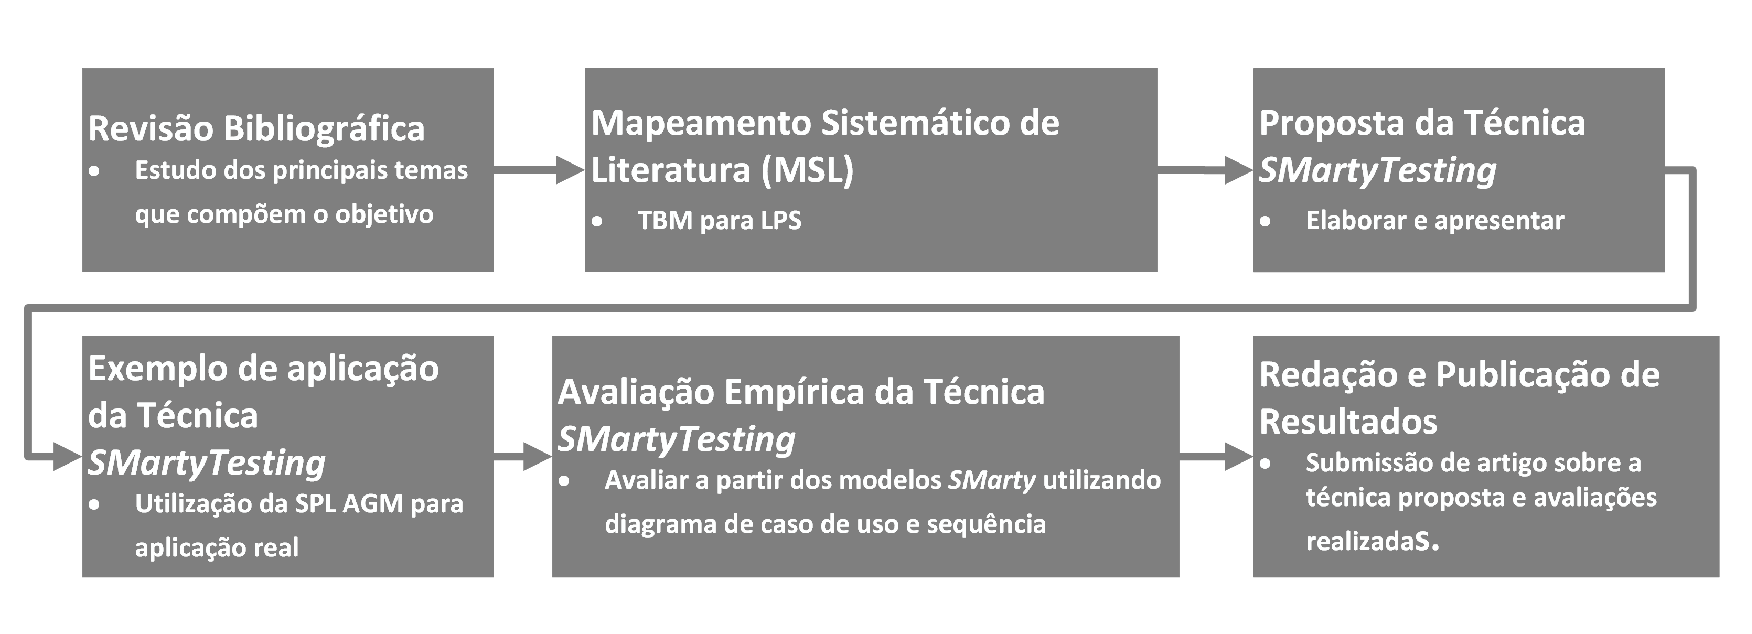
\includegraphics[scale=0.40]{fluxo_metodologia.pdf}
	\caption{Etapas da Metodologia de Desenvolvimento de Pesquisa}
	\label{fig:fluxometodo}
\end{figure}

\begin{itemize}
	\item \textbf{Revisão Bibliográfica:} Estudo dos conceitos sobre os principais temas que farão parte do objetivos da pesquisa, como: Perfis UML, Diagramas de caso de uso e sequência, teste em LPS, TBM, conceitos de LPS, gerenciamento de variabilidade, a abordagem \textit{SMarty} que está no Anexo \ref{Abordagem_SMarty}. 
	
	\item \textbf{Estudo secundário:} Realização de uma Revisão Sistemática de Literatura (RSL), de estudos primários, onde o tema é TBM para LPS, que encontra-se no Apêndice \ref{sec:MSL}. A análise dos estudos da RSL permitiu a identificação de formatos diferenciados de aplicação de TBM em LPS.
	
	\item \textbf{Proposta da Técnica \textit{SMartyTesting}:} Elaborar e apresentar a proposta da técnica \textit{SMartyTesting} que visa a utilização de TBM para LPS modeladas usando \textit{SMarty} para geração de casos de teste em nível de sistema a partir de um modelo formal.
	
	\item \textbf{Exemplo de aplicação da Técnica \textit{SMartyTesting}:} Utilização da LPS acadêmica \textit{Arcade Game Maker}(AGM) para aplicar a técnica \textit{SMartyTesting} para a aprendizagem dos conceitos de SPL através de uma abordagem prática. Esta LPS pode ser usada para derivar três jogos eletrônicos diferentes; Bowling, Brickles e Pong, que são usados pela comunidade científica para avaliar e validar suas abordagens \textcolor{red}{colocar uma referencia de onde ele pode obter a lps AGM} \cite{costa2016split}.
	
	\item \textbf{Avaliação Qualitativa da Técnica \textit{SMartyTesting}:} trata dos estudos empíricos que serão conduzidos com a finalidade de validar \textit{SMartyTesting} em relação a geração de casos de teste a partir de modelos \textit{SMarty} utilizando-se de diagrama de caso de uso e sequência. Nas avaliações serão utilizadas as LPS \textit{Mobile Media}(MM) e M-SPLlearning ** ou plets.
	
	\item \textbf{Redação e Publicação de Resultados:} é escrita e submissão de artigos sobre a técnica proposta e os estudos empíricos conduzidos, bem a escrita e publicação sobre a RSL gerada como estudo secundário, além da escrita e defesa da dissertação.
	
	
\end{itemize}

\subsection{Ciclo de Desenvolvimento}

contextualizar o ciclo de teste pesquisado

posicionar o leitor onde esta nossa abordagem

\subsection{RoadMap teste TBM em LPS}

apresenta o os caminhos possíveis encontrados no mapeamento e o qual foi o escolhido e porque



\subsection{Conversão de Sequência para Atividade}
apresentar o motivo de diagrama de sequencia ser o escolhido

porque a conversão para atividade

possibilidade de conversão para maquina de estado

apresentar de forma detalhada o mapeamento



\subsection{Geração de Sequências de Teste}

falar o que é geração de sequencia de teste

falar sobre os metodos de geração de sequencia W, HSI etc

falar sobre a ferramenta plavis

apresentar como é o processo da split mbt

explicar o porque foi escolhido a split



\subsection{Feramentas Adaptadas (SPLit-MbT)}

porque foi selecionado a split e todos os detalhes de seu funcionamento


\subsection{Ferramentas e Caminho Escolhido *****}
Neste trabalho estamos em análise para algumas ATLs de conversão, uma para a primeira etapa \textit{Convert UML Sequence Diagram to UML State Machine } que está sendo testada, e uma para a segunda,  já a segunda deverá ser implementada, devido as particularidades da geração de sequência de teste contendo variabilidade, além da ATL, outras ferramentas estão sendo utilizadas, como o Eclipse, UML \textit{Designer}. A \ref{fig:roadmap} apresenta o caminho que optamos dentro do contexto levantado pelo mapeamento sistemático da literatura apresentado no Anexo \ref{sec:MSL}.


\begin{landscape}
	
	\begin{figure}[htb]
		\centering
		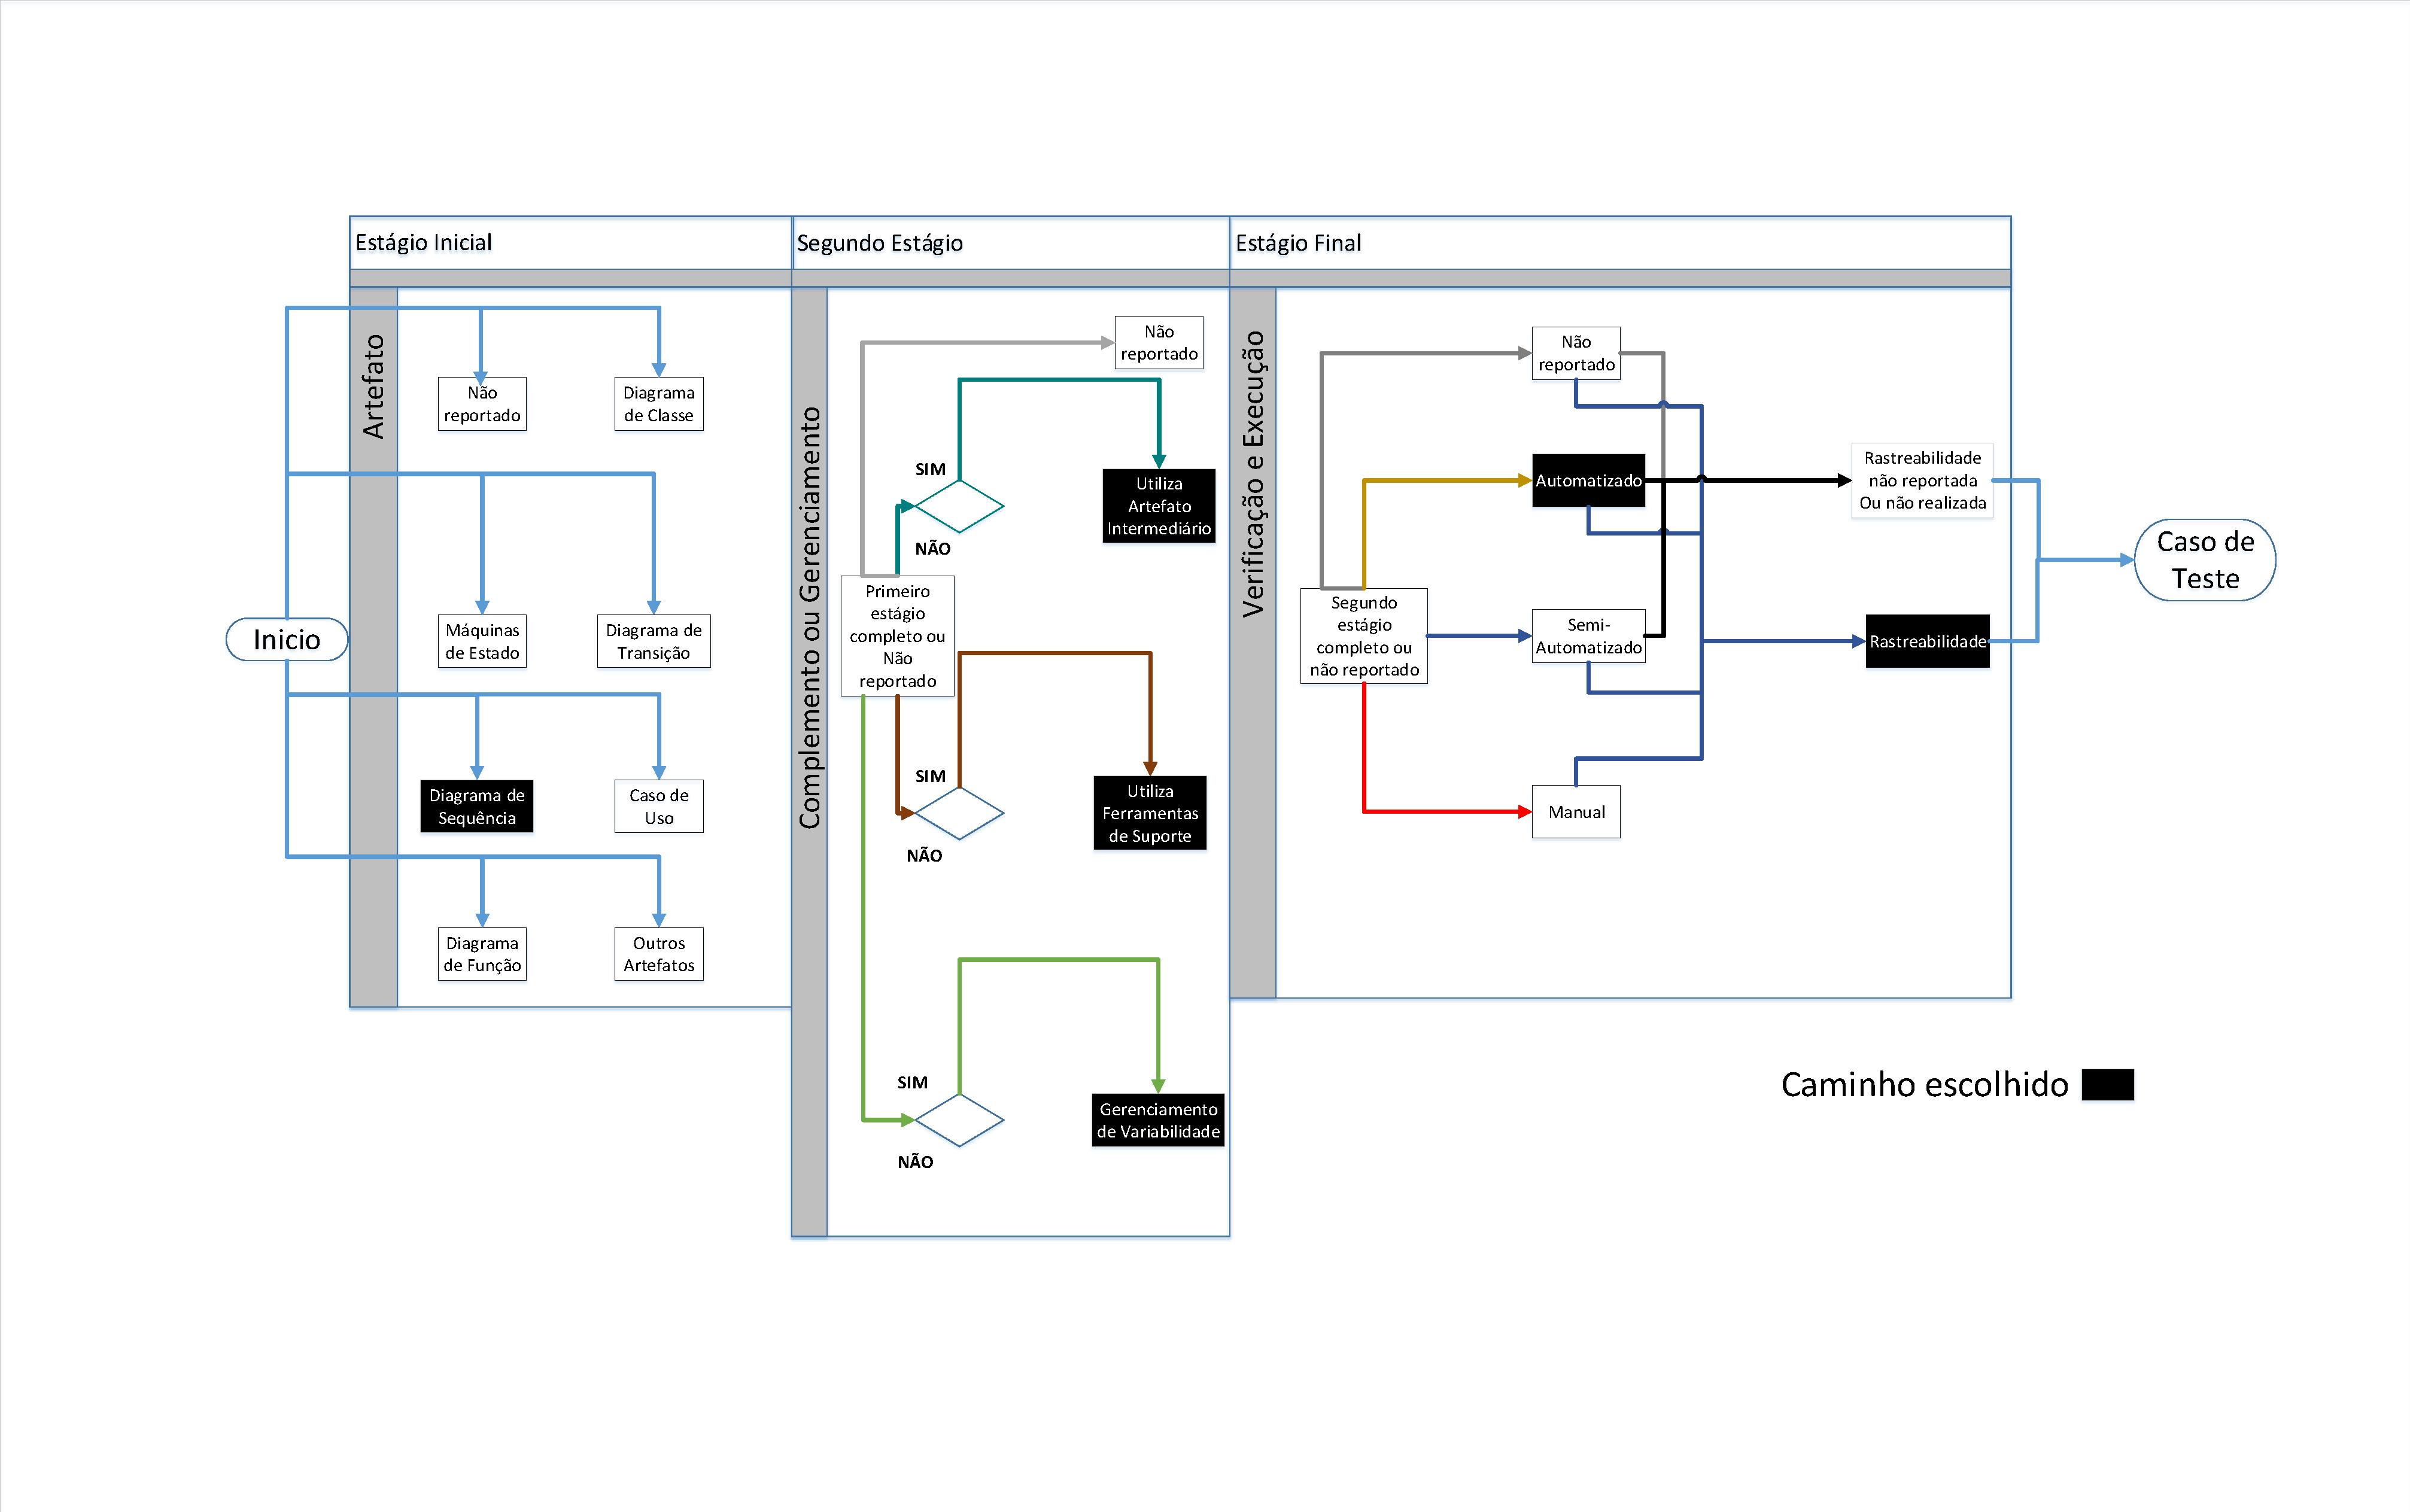
\includegraphics[scale=0.30]{road_map.pdf}
		\caption{Guia de direcionamento de processo de TBM em LPS}
		\label{fig:roadmap}
	\end{figure}
	
\end{landscape}




\subsection{Desafios Encontrados}
A literatura apresenta muitas soluções para teste de LPS, porém muitas delas não possuem foco na variabilidade quando o assunto é uma LPS. Assim, um dos fatores motivantes é considerar variabilidade na decisão de teste. Outro ponto motivante é a abordagem \textit{SMarty} \cite{junior2010systematic} que permite a representação de variabilidade em modelos iniciais do ciclo de vida de LPS. Quando se fala em teste, a literatura apresenta várias soluções voltadas a LPS, dentre elas o TBM, embora trabalhe com MEF, seria interessante que pudesse ser trabalhado o teste com artefatos do tipo casos de uso, diagramas de sequência e de atividades, além de diagramas de estado que já é bastante utilizado. Assim, entende-se como uma oportunidade que pesquise o TBM em conjunto \textit{SMarty} para utilização em casos de uso e diagrama de sequência, para se obter casos de teste que possam ser utilizados a nível de sistema.

\citealp{costa2016split, olimpiew2008model} apresentam alguns desafios na geração de testes a partir de modelos em uma LPS, um ciclo de criação que perfaz desde o modelo inicial até o caso de teste. Devido as particularidades de cada modelo, se faz necessário adaptações a respeito, um exemplo é onde \citealp{costa2016split} estende a máquina de estado finito, pois ela não possui suporte para variabilidade e para garantir que a variabilidade fosse mantida isso se fez necessário. \citealp{olimpiew2008model} também faz de forma semelhante a em sua abordagem CaDeT, modificando parte dos itens para poder contemplar o objetivo da proposta.

\textit{SMartyTesting} não seria diferente, houve a necessidade de se encontrar ferramentas que fizessem o apoio automatizado do processo. Sendo assim buscamos procurar a linguagem de transformação de modelos é usada para definir como um conjunto de modelos de origem é mapeado com o objetivo de criar um conjunto de modelos de destino. A linguagem define como as operações básicas sobre os modelos podem ser realizadas usando um conjunto especíco de construções de linguagem. A criação de linguagens especícas para transformação de modelos é uma abordagem que foi tomada pela indústria de software e comunidade de pesquisa. Como resultado,diversas linguagens de transformação de modelos têm sido propostas \citealp{allilaire2006atl}.

\subsubsection{Limitações de Uso}

apresentar as limitações de uso em relação a pesquisa e os suportes que as ferramentas possuem

limitações do mapeamento e da split

\subsubsection{Ameaças ao Funcionamento}

apresentar as ameaças relacionadas as limitações de uso e interpretação do usuário

Mesmo havendo um embasamento de todo o estudo apresentado aqui a partir da MSL, ainda podemos constatar que podem surgir ameaças ao funcionamento da abordagem quando o assunto é a conversão dos artefatos. Por optarmos trabalhar com diagramas de sequência como ponto de partida, a ATL de conversão trabalha com um metamodelo UML, se o arquiteto de software modelar diagramas que não atendem a quantidade minima de informações necessárias no diagrama, isso pode mascarar itens, ou criar processos equivocados. Um exemplo seria a representação de um laço de repetição de forma diferente do convencional, que da forma como for representado o retorno, poderá gerar uma sequencia de teste como uma outra operação diferente de um laço de repetição. Sendo assim, devemos apresentar ao utilizador um padrão mínimo para que a seja obtido o resultado esperado.


\section{Especificação da Abordagem SMartyTesting}
\label{especificacao_smarty}
Nesta Seção é apresentado de forma mais detalhada a abordagem \textit{SMartyTesting}, para um bom entendimento se faz obrigatório a leitura da Seção \ref{caracterizacao_smarty}.

\subsection{Etapa 1 - Mapeamento de Diagrama de Sequência para Diagrama de Atividade}

explicar de forma detalhada o mapeamento de sequencia para atividade





Como mencionado na Seção \ref{sec:porque_sequencia} a opção por diagramas de sequência se deve ao fato de ele possibilitar uma maior riqueza de informações a respeito do modelo.
A escolha por diagrama de estado na geração de sequência de teste se deve ao fato de ele ser um dos modelos formais mais utilizados em TBM. Além disso ele é uma boa alternativa para projetar componente de teste, pois podem ser aplicáveis em qualquer modelo de especificação descrevendo um número finito de estados, outro ponto é que ele também é o mais adequado para gerar sequências de teste, uma vez que optamos por esse caminho \cite{costa2016split}.


\subsection{ATLs de Conversão UML}

falar sobre algumas ATLs de conversão e os limitadores da utilização deste recurso

Foram encontradas duas ATLs de conversão a primeira \textit{UML Sequence Diagrams to Statechart Diagram} \footnote[1]{Disponível em:http://www.st.ewi.tudelft.nl/basgraaf/ - Acessado em 20/03/2019} onde a documentação de utilização é extremamente confusa e de difícil configuração, foram feitos tentes de conversão de diagramas de exemplos que estavam no pacote, mas não foi obtido o resultado esperado. Já a segunda também \textit{open-source}, é chamada de \textit{Convert UML Sequence Diagram to UML State Machine} \footnote[1]{Disponível em: https://github.com/slashburn/mdd-project - Acessado em 10/04/2019} que possui uma documentação um pouco mais detalhadas em comparação a anterior, foram realizados teste iniciais com os exemplos contidos no pacote onde ouve exito de conversão \cite{hennicker2007activity}.

Este pacote utiliza uma linguagem de conversão \textit{Query/View/Transformation} (QVT), QVT é uma linguagem usada para transformar (meta) modelos. Ele usa OCL (Linguagem de Restrição de Objeto) estendida em combinação com uma linguagem específica de domínio: Relações, Core ou Operacional. Este último é uma linguagem imperativa, enquanto os outros dois são declarativos, ela é implementada no Eclipse.

\textit{Convert UML Sequence Diagram to UML State Machine} possui suporte a arquivos com extensão UML, sendo assim a quantidade de ferramentas que poderiam auxiliar na concepção de diagramas que pudessem ser convertidos ficou um pouco limitada, devido a outras existentes utilizarem formatos próprios de saída, a princípio não realizamos uma busca por conversões de formato para obter uma abrangência maior, ao invés disso procuramos uma ferramenta que fosse robusta e pudesse entregar o proposto. Sendo assim, optamos por realizar testes como o \textit{UML Designer}  \footnote[2]{Disponível em: http://www.umldesigner.org/download/ - Acessado em 10/04/2019}.

\subsubsection{Convert UML Sequence Diagram to UML State Machine}
\textit{Convert UML Sequence Diagram to UML State Machine} se mostra compatível com \textit{SMarty}, pois em sua conversão apresenta um arquivo de extensão \textit{notation} ainda não foram realizados testes com artefatos modelados por \textit{SMarty} mas baseado nas documentações o resultado pode ser satisfatório. Na \ref{fig:SM_etapa1} apresenta uma visão do ciclo da primeira etapa de forma mais resumida, sendo assim na primeira etapa ficou definido a seguinte sequência de ações, onde grande parte automatizada. 

Partindo do pressuposto que o artefato seja diagrama de sequência e também modelado no formato \textit{SMarty}, é feito a entrada do artefato em extensão UML, na IDE eclipse através da ATL \textit{Convert UML Sequence Diagram to UML State Machine} é realizado as configurações pré-definidas e após a conversão é gerado dois arquivos, um com extensão \textit{notation} e outro UML.


\begin{figure}[htb]
	\centering
	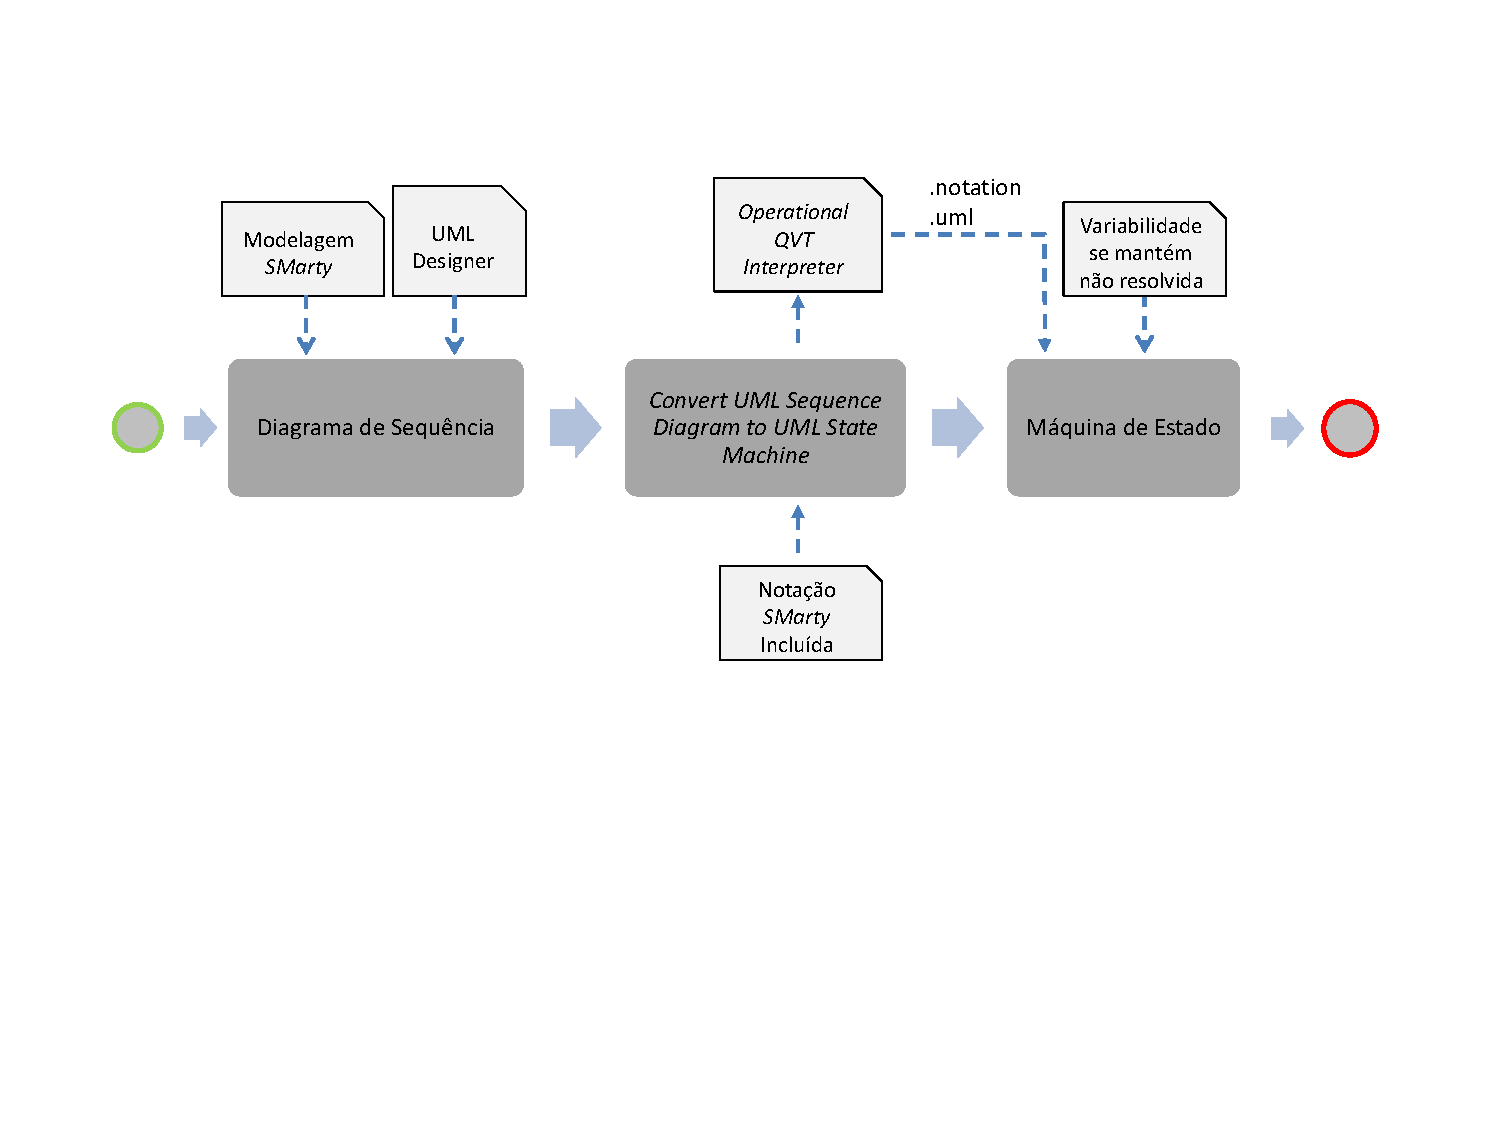
\includegraphics[scale=0.50]{smartytesting_etapa1.pdf}
	\caption{Ciclo da etapa 1}
	\label{fig:SM_etapa1}
\end{figure}


\subsection{Etapa 2 - Geração de Sequência de Teste com apoio da ferramenta SPLit-MbT}
\label{etapa2}

explicar de forma detalhada a geração da sequencia de teste utilizando a split


Após a conversão do artefato para máquina de estado contendo a variabilidade, idealizamos a geração de sequências de teste, onde será possível verificar todas as possíveis combinações e coberturas do artefato. O desafio inicial é como realizar a geração de sequência de teste a partir de máquina de estado, para isso desenvolvemos uma pesquisa a respeito. Realizamos também uma análise para entender se seria vantagem a geração de caso de teste diretamente do artefato de máquina de estado, onde poucos trabalhos foram reportados \cite{aggarwal2012test,dalepiane2014implementation,samuel2008automatic}, porém, nenhuma deles aborda LPS. 

Na busca por modelos de conversão \citealp{costa2016split} relata os principais métodos com suporte a diagrama de máquinas de estado,  TT, UIO, DS, W or HSI, porém alguns deles não seriam possíveis de utilização em LPS, no estudo ele relata que o HSI foi o método que contém mais características favoráveis a utilização em LPS. Também um dos métodos menos restritivos em relação às propriedades que as máquinas de estado devem ter, outro detalhe é que, iremos realizar uma avaliação para comparar os dados obtidos com o trabalho de \citealp{costa2016split}. 

Um outro exemplo é que o HSI é capaz de interpretar MEF completas e parciais.sendo assim, iremos buscar implementar tal método para geração de sequências de teste através de diagramas de máquinas de estado.

\begin{figure}[htb]
	\centering
	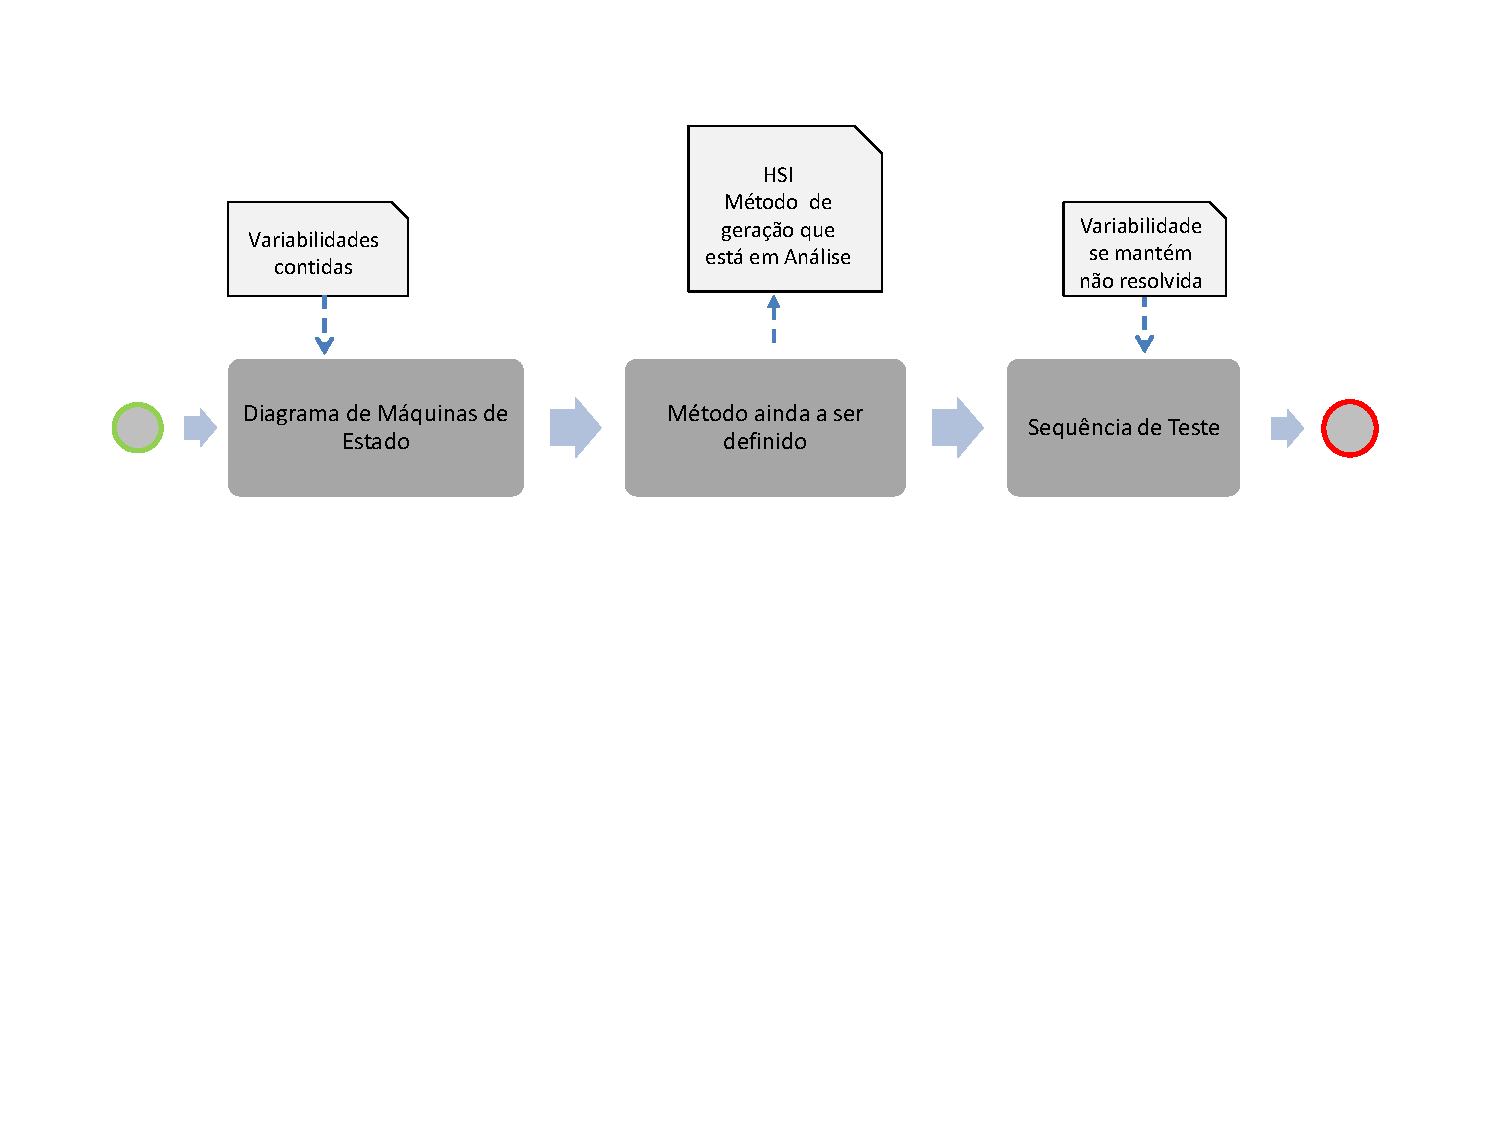
\includegraphics[scale=0.50]{smartytesting_etapa2.pdf}
	\caption{Ciclo da etapa 2}
	\label{fig:SM_etapa2}
\end{figure}


\subsection{Solução da Variabilidade na Engenharia de Domínio}

explicar que a variabilidade fica para ser resolvida na engenharia de aplicação

Um dos objetivos deste trabalho é o gerenciamento da variabilidade na geração dos casos de teste. Analisando estudos resultantes da MSL no Anexo \ref{sec:MSL} observamos que quando se abordado produtos derivados a variabilidade sempre é deixada para ser resolvida na engenharia de aplicação, principalmente se houver o interesse no reaproveitamento do caso de teste. Pois um dos principais argumento é que se houver o reaproveitamento pode haver leves variações no ponto de variabilidade o que implicaria em um retrabalho na solução da variabilidade já resolvida.

Seguindo essa premissa, o caso de teste será gerado contendo a variabilidade, sem a solução. Estará documentado a variabilidade e suas particularidades, mas sem a solução devida, ficando a cargo do responsável em qual etapa da engenharia de aplicação será realizada a solução. 


\section{Exemplo de Aplicação}
\label{exemplo_aplicao_smarty}

ilustrar a utilização com um diagrama

\section{Considerações Finais}
\label{consideracoes_smarty}
